\chapter{Ransomeware}\label{Ransomeware}

In this chapter we talk about the theoretical background of ransomeware.
First we start with a few general definition and then we discus the general workflow of ransomeware.


\section{Definition}\label{Definition}

\subsection{Malware}

Malware is the short term for `malicious software', which refers to the software programs, who are designed to damage or do other unwanted actions on a computer system \cite{malware}. We have all kinds of malware for example: viruses, worms, trojan horses, and spyware. For this project we are focussing on another type of malware namely, ransomeware.

\subsection{Ransomeware}

Ransomeware is a type of malware, which hijacks the files on the infected computer by encryption all the files. The only way the ransomeware will decrypt the files, is when the victim pays the asked ransom money. The strength of the encryption and asked ransom money vary, but as we will see in the next section, every ransomeware has the same general pattern. They only differ in the tweaks they apply in those main components.

\section{Workflow}\label{workflow}

In this section we take a closer look at the workflow of the ransomeware. In every type of ransomeware we find the same workflow. Every ransomware starts with the search for a victim. After finding a victim it has to look for a weak spot, which makes it possible to install the ransomeware. When the weak spot is found, the ransomware installs itself and hijacks the files of the victim by encryption. After the completion of the installation the ransomeware notifies the victim and asks for ransom money. Only when the ransom is paid, the ransomeware will decrypt the files of the victim.

In the next subsections we talk about each step of the workflow in greater detail.

\subsection{The Search For A Victim}\label{search}

The first step you need to do, when a criminal wants to use ransomeware is finding a victim. Nowadays with the internet is this very. A criminal can get in touch in several ways.

\subsubsection{E-mail}

A popular way is by email. Most of the time criminals craft an email with social engineering techniques, which causes the victim to open the attachment in the email. This attachments seems harmless for the victim but is in reality the ransomeware, which immediately infects the victim's computer when opened.


\begin{figure}[H]
    \centering 
    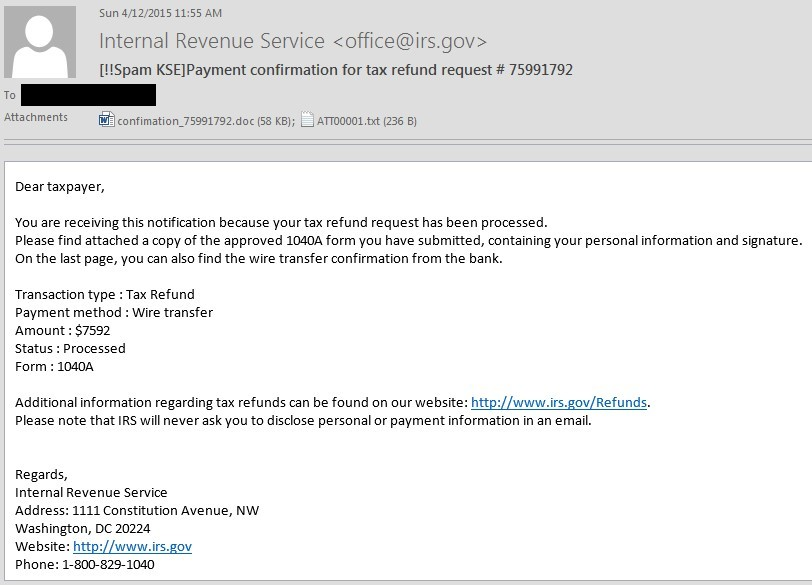
\includegraphics[height=7cm]{example_ransomemail}
    % \caption{An example of a specially crafted email by a criminal, which causes the reader to open the attachment.
    \caption[]{An example of a specially crafted email by a criminal, which causes the reader to open the attachment.\protect\footnotemark}
    \label{ransomemail}
\end{figure}
\footnotetext{Source: http://i1-news.softpedia-static.com/images/news2/Users-in-the-US-Targeted-with-Ransomware-Via-Tax-Return-Flavored-Emails-478465-2.jpg}

\subsubsection{Removable Device}

Another methode is a removable device. This can be a USB-stick, CD or even a mobile phone. The device can be plugged in by the criminal himself or he let lying around intentionally some removable devices in the hope the finder would connect it with the computer.

In the next section we will take look at how we can trick the victim in activating the ransomeware.

\subsection{Tricking the victim}\label{theorie_trick}

As we said in section \ref{search} we can reach a victim in several ways. But reaching the victim is not enough. The ransomeware has still to execute.\\

If we want for example to reach the victim by email. The user can not have any clue that the attachment is malicious and has to have the intention to open the ransomeware. A possible trick is \textbf{Obfuscation the executable}.

\subsubsection{Obfuscation The Executable}

Like we already said, we do want the victim to open the ransomeware.A possible methode is obfuscation the executable. We want to look our file as harmless as possible. The best way to do obfuscate your ransomeware as a widely used file, for example a pdf.
To obfuscate our file we can use two little tricks. First we can change the icon of our executable in the typical icon used for that fileformat. Next we can rename our ransomeware from \textit{thisisnotevil.exe} to \textit{thisfileisnotevil.pdf.exe}. 
Now when the user has is security settings on standaard, which is on default, the victim will see a harmless file called \textit{thisfileisnotevil.pdf} with a familiar icon.


\subsection{Compromising The Victim's Machine}\label{Compromising}

After having access to the system, the next logical step is compromising the victim's machine. In the case of ransomeware is this encryption of the files. In the first generations of ransomeware, self-written encryption algorithms were used. Because they were self-written the encryptions were often crackable. However the malware designers got smarter and the ransomware of nowadays uses the public available encryption libraries, which are unfortunately less or not crackable.

\subsection{Notifying The Victim}\label{notify}

After compromising the victim's machine, a characteristic feature of ransomeware is notifying the victim.\\
\\
Also here do we see a evolution throughout the years. With the first generations the victim got completely locked out of his system. Although after a while criminals discovered it is better to still grant access to the system and confront the victim with the encrypted files. Because the victim still sees the encrypted files, the victim is more willing to pay the ransom. This is why ransomeware of today only encrypt the personal files and not the whole system. \\
\\

Further happens the notifying by changing the background and putting two files on the desktop, one is a list with the encrypted files, again to confront the victim. And the other file is a instruction file with further instructions for the victim to decrypt his files.\\
\\

At last is it often the case the victim is put under pressure with a countdown timer. By this timer the criminal threatens that if the countdown timer ends, the files will be unrecoverable.

\subsection{Decryption}\label{decryption}

After the ransom is paid the user can follow up the instructions of the readme file and download the decryption software. Only with this software is it possible to decrypt the encrypted files.
